% #############################################################################
% This is Chapter 3
% !TEX root = ../main.tex
% #############################################################################
\fancychapter{Hybrid models for children automatic speech recognition}
\label{chap:Chapter3}
\cleardoublepage
\section{Introduction}
% HMM-DNN played a signifant role in ASR (quick history recap)
In the history of ASR, HMM-based models emerged as a popular choice for acoustic modeling since the 1980s. The application of HMMs offered a structured framework to effectively model the temporal dependencies inherent in speech signals.The initial paradigm involved combining HMMs with GMMs to represent the probability distributions of acoustic features. This traditional HMM-GMM architecture, while effective to a certain extent, faced limitations in capturing the intricacies of complex, non-linear relationships present in speech data. Therefore, a pivotal turning point occurred with the integration of DNN, evolving towards hybrid HMM-DNN models. This paradigm shift lead to substantial improvements in ASR performances. Inded, DNNs brought enhanced modeling capabilities, allowing the system to discern more nuanced acoustic patterns and adapt better to diverse linguistic contexts. The hybrid HMM-DNN approach has become key architecture in modern ASR systems, demonstrating remarkable success in handling large vocabulary tasks and challenging acoustic conditions \cite{!!}. 

% Why HMM-DNN for children
In Chapter \ref{chap:Chapter2}, we saw how a HMM-GMM or HMM-DNN ASR system can directly integrate relevant knowledge into the ASR pipeline. This knowledge is transmited to the pipeline using the language model, acoustic model, and vocabulary. Having hand-crafted knowledge directly in the ASR system allows to reduce the amount of speech data required to generate appropriate results. Such characteristics was found beneficial for children ASR where the amount of data is limited. According to the literature, a common family of methodologies  found to be benefits in improving ASR results are the inductive bias approaches such as transfer learning and multi-task learning \cite{TransferLF}. For years, HMM-based configurations have been a privileged setting for the children's ASR community. As a matter of fact, between 2009 and 2020, 80\% of published research on children's speech recognition was based on hybrid systems, with 45\% using HMM-GMM and 35\% HMM-DNN. However, one notable observation was that during the same period, 63\% of published work was conducted for English \cite{big_review_childASR}. As a result, it is uncertain how children's speech from other languages relates to the various approaches used in English, particularly transfer and multi-task learning.

% What we planned to do here
In this chapter, we will first present the factorised time delay neural network (TDNN-F) in HMM-DNN ASR system as our system relies on it. Then, we will delve into applying knowledge transfer strategies applied across various scenarios, encompassing both non-English and English datasets. Applying it to non-English dataset will allow us to understand if inductive bais approaches are still working in the context of non-English children speech. To this end, we present an examination of transfer and multi-task learning methodologies, leveraging adult speech as an inductive bias, a prevalent approach in the existing literature. 

Finally, as our contribution, we introduce a novel approach termed "multilingual transfer learning". This strategy integrates both transfer and multi-task learning techniques, where we address the challenge posed by the scarcity of data for both adult and children's in low-resource languages by using the combination of transfer and multi-task learning methodologies but restrict our focus solely to low-resourced  children's speech datasets.
%aiming to obtain a better ASR model for children.
%This chapter will investigate these strategies in a variety of scenarios employing non-English data and English data. First, we present transfer and multi-task learning using adult speech as an inductive bias, as is common in the literature. Second, because there is a lack of data for both adult and children's low-resource languages, we investigate the same methodologies using only children's speech. Finally, we present our approach, multilingual transfer learning, which combines transfer and multi-task learning to produce a more robust model for speech recognition in low-resource children setting.

\section{Factorised Time Delay Neural Network for children ASR}
\label{sec:TDNNF}
\begin{figure}[ht]
    \centering
    \subfigure[TDNN with sub-sampling]{\label{fig:tdnn}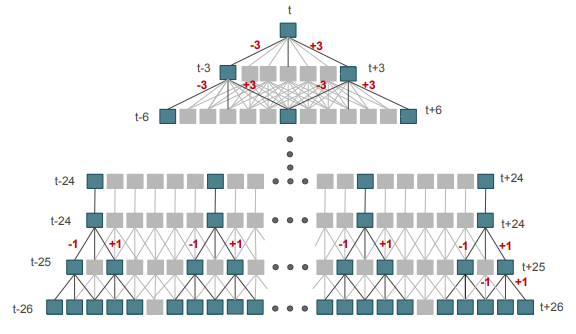
\includegraphics[width=0.49\textwidth]{imgs/TDNN.png}}
    \subfigure[Factorised TDNN layer]{\label{fig:tdnnf}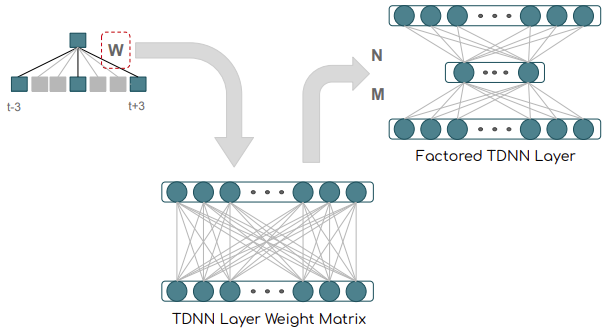
\includegraphics[width=0.49\textwidth]{imgs/TDNNF.png}}
    \caption{TDDN and TDNN-F taken from \cite{tdnnf-children}}
\end{figure}
% Focus on this section
In this chapter, we will focus on the application of HMM-DNN-based models, specifically leveraging the Factorised Time-Delay Neural Network (TDNN-F) architecture.  Instead of revisiting the entire HMM-DNN framework, extensively covered in Chapter \ref{chap:Chapter2}, we will delve into the distinctive features of the DNN architecture employed for the rest of this chapter, namely the TDNN-F. 
The use of the TDNN-F architecture was motivated by the need to improve ASR performances in scenarios characterised by limited speech data and its successful use for children ASR \cite{tdnnf-children}. This choice aligns with the broader trend in ASR research where there is increasingly interest to explore more data-efficient neural network architectures, with the TDNN-F standing out as a notable example.

% How TDNN works
In a traditional TDNN, the input at time step $t$ is send to the next layer along with its neighboring frames within a specific context window \cite{tdnn}. The network's depth enables the TDNN to integrate information over a broader context window. However, this design can lead to computational inefficiency due to the context windows for adjacent steps overlap. Therefore, as illustrated in Figure \ref{fig:tdnn}, an alternative approach is to sub-sample the input sequence, which means skipping same frames, and transmit only the sampled frames. This sub-sampling technique offers a trade-off between computational efficiency and the network's ability to capture temporal dependencies. Indeed, by selectively processing a subset of frames, the TDNN can maintain its ability to capture relevant information while reducing the computational cost associated with processing every frame.

% How TDNN-F works
The TDNN-F architecture \cite{TDNN-F} enhances the TDNN by improving the computational efficiency of the network. This is achieved by decomposing the weight matrix of each TDNN layer into an approximation as the product of two lower-rank matrices using SVD, defined as:
\begin{equation}
    \text{W} = \text{U}\Sigma \text{V}^T = \text{MN}
\end{equation}
Here, $\Sigma \in \mathbb{R}^{m \times n}$ is a non-negative rectangular diagonal matrix, and $\text{M} \in \mathbb{R}^{m \times k}$ and $\text{N} \in \mathbb{R}^{k \times n}$ with $k \leq \min(m,n)$. The goal is to ensure that one of the two sub-matrices is close to a semi-orthogonal matrix, representing either $\text{U}\Sigma$ or $\Sigma \text{V}^T$. Notably, $k$ is typically chosen to be much smaller than $m$ and $n$.
During the training of the network, after every few updates of the entire network, a specific update is performed on matrix $\text{N}$ using Stochastic Gradient Descent (SGD). This update is guided by an additional objective function, which ensures that $\text{N}$ is not too far from being semi-orthogonal.
The introduction of the semi-orthogonal constraint through the matrix factorisation process in TDNN-F can be viewed as adding an extra bottleneck layer to the traditional TDNN. A visual representation of the TDNN-F layers is presented in Figure \ref{fig:tdnnf}. This bottleneck layer, represented by the reduced-rank matrix $\text{N}$, contributes to the overall efficiency of the network by reducing the number of parameters and computations required while preserving essential information.


\section{Assessing the efficacy of multi-task and transfer learning from adult to children}
\label{section:HMMDNNADULT2CHILD}
\subsection{Methodology}

% Motivation
Motivated by the success of knowledge transfer approaches for children ASR using adult data as inductive bias in the literature \cite{TFchildren,TransferLF,2019multi}, we intend to extend and validate these findings using a low-resource language. The reason behind leveraging adult data for pre-training lies in the stability and reduced variability found in adult speech. This characteristic simplifies the extraction and recognition of intrinsic and meaningful speech patterns.
Therefore, we proposed to assess children's speech recognition performances in four distinct configurations:
\begin{enumerate}
    \item \textbf{Adult model}: Training a model from scratch using only adult data. This configuration serves as a baseline to assess the standalone performance of a model trained exclusively on adult speech.
    \item \textbf{Children model}: Training a model from scratch using only children's data. This configuration provides insights into the model's ability to learn from children's speech without leveraging adult data.
    \item \textbf{Multi-task model}: Training a model concurrently on adult and children data using multi-task learning. This configuration explores the potential benefits of simultaneous training on both adult and children data.
    \item \textbf{Transfer learning}: Fine-tuning a model on children's data that was pre-trained on adult data (from the Adult Model in Configuration 1). This configuration assesses the effectiveness of transferring knowledge from adult to children data for improved speech recognition.
\end{enumerate}

By systematically comparing these configurations, our objective is to identify the most effective approach for enhancing ASR performance in children ASR, particularly in low-resource language scenarios and answering the research question  \textit{Which knowledge transfer approach is best for efficiently modelling and improving automatic recognition of children's speech?} 


\subsection{Corpus}
\label{sec:corpus}
In our evaluation of children's speech performance in a low-resource language context, we have chosen European Portuguese as our target language. European Portuguese qualifies as a low-resource language due to the limited availability of large-scale adult speech corpora, with most datasets not exceeding 100 hours \cite{tribus}. For this experiment, we used the LetsRead child corpus, detailed in Section \ref{section:children_corpora}, to represent children's speech in European Portuguese. Additionally, we employed the BD-PUBLICO corpus as the adult counterpart. The statistics of both corpora are presented in Table \ref{tab:statistics_exp1}.
%As stated in the introduction, we aim to evaluate the performance of children's speech in a low-resource language. To this end, we decided to use European Portuguese corpora. European Portuguese can be considered a low-resource language since most adult speech corpora do not exceed 100 hours \cite{tribus}.
%In this experiment, we used LetsRead, a child corpus, described in section \ref{section:children_corpora} and BD-PUBLICO as adult corpus. %However, given the relatively small size of BD-PUBLICO, we chose to expand our experiments with a large English corpus, Librispeech-960. 
%The statistics of all these two corpora are provided in the following table \ref{tab:statistics_exp1}. The rest of this section provides further information about the BD-PUBLICO corpus.%these two adult corpora.

% Stat corpus 
\begin{table}[h]
\begin{center}
\begin{tabular}{lcc}
\hline
Corpus name      & Train & Test  \\ \hline
\multicolumn{1}{l}{BD-PUBLICO}             & 8085 utt  & 412 utt  \\ 
\multicolumn{1}{c}{\textit{Adult}}              & 21h48 & 01h10 \\\hline
\multicolumn{1}{l}{LETSREAD}     & 3590 utt & 1039 utt \\ 
\multicolumn{1}{c}{\textit{Children}}     & 12h00 & 02h30 \\  \hline
%\multicolumn{1}{l}{Librispeech}                     & 281241 utt &   \\ 
%\multicolumn{1}{l}{}      &                &  960h &  \\ \hline
\end{tabular}
\caption{Number of utterances and duration of the different corpora for multi-task and transfer learning experiments using adult and children data}
\label{tab:statistics_exp1}
\end{center}
\end{table}

\subsubsection*{BD-PUBLICO}
The BD-PUBLICO database (Base de Dados em Português eUropeu, vocaBulário Largo, Independente do orador e fala COntínua) \cite{bdpublico} consists of reading sentences extracted from the Portuguese newspaper PÚBLICO over a 6-month period, the corpus encompasses linguistic diversity with 10 million words and 156,000 different forms. Recordings involve 120 speakers, specifically graduate and undergraduate students from Instituto Superior Técnico (Lisbon), all falling within the age range of 19 to 28 years, establishing BD-PUBLICO as an adult dataset. Recordings occurred in optimal noise conditions within a soundproof room at INESC-ID (Lisbon), with a sampling frequency of 16kHz and the use of a high-quality microphone. The corpus includes a pronunciation lexicon with citation phonemic transcriptions, with manual corrections applied to enhance transcription accuracy.

For effective model training and evaluation, we partitioned the BD-PUBLICO corpus into three distinct sets, ensuring balanced gender distribution. The training set comprises 80 sentences performed by each of the 100 speakers. The development set, consisting of 40 sentences performed by 10 speakers. Finally, the test set includes 40 sentences performed by 10 speakers.


%The BD-PUBLICO database (Base de Dados em Português eUropeu, vocaBulário Largo, Independente do orador e fala COntínua) \cite{bdpublico} consists of reading sentences extracted from Portuguese newspaper PÚBLICO. The sentences that are read correspond to a total of 6 months of news (equivalent to 10M words and 156k different forms). It is composed of 120 speakers, and graduate and undergraduate students from Instituto Superior Técnico (Lisbon). This corpus is considered an adult dataset since all students are between 19 and 28 years old. All recordings were performed in good noise condition, in a soundproof room at INESC-ID (Lisbon), at a sampling frequency of 16kHz and using a high-quality microphone. In addition, a pronunciation lexicon with citation phonemic transcriptions for each word was produced. Finally, manually corrections were applied to the automatically generated transcriptions. 

%We divided the BD-PUBLICO corpus into three unique sets with balanced gender partitioning: 1) A training set of 80 sentences by 100 speakers. 2) A development set of 40 sentences performed by a total of 10 speakers. Finally, a test set of 40 sentences by 10 speakers.

%\subsubsection*{Librispeech}
%Librispeech corpus is one of the biggest publicly available speech dataset \cite{librispeech}. It is a collection of 982 hours recorded at 16kHz from 2484 adult speakers derived from audiobooks. Librispeech corpus is designed to ensure a gender balance and no speaker overlap between train, development and test sets.


\subsection{Experimental setup}
\label{section:exp_setup}

All experiments were conducted using the Kaldi open-source toolkit \cite{kaldi}. Initially, for each corpus, an independent HMM-GMM acoustic model was trained to generate the necessary alignment for the subsequent HMM-DNN model. Subsequently, HMM-DNN acoustic models were trained using 40-dimensional fbanks alongside 40-dimensional Spectral Subband Centroid (SSC) features \cite{ssc}. The inclusion of SSC features, which share properties with formant frequencies, is anticipated to enhance vowel recognition and contribute to improved recognition of children's speech. The resulting 80-dimensional input features were augmented by a 100-dimensional speaker embeddding i-vector. Concatenating speaker embeddings to the input features is commonly employed to enhance model speaker robustness in HMM-based model \cite{ivector}. Our i-vector extractor was specifically trained on a pooled set of children's data, encompassing LetsRead, PfStar Swedish, Etltde, Cmu kids, and Chorec, as described in Section \ref{section:children_corpora}.

To augment the training corpora, data augmentation techniques were applied, including perturbing the speaking rate of each training utterance by factors of 0.9 and 1.1, as well as volume perturbation. This augmentation strategy enhances the network's robustness to variations in speaking rate and volume during testing. Additionally, Specaugment \cite{specaugment} was employed on top of the fbanks and SSC features, involving random masking of time and frequency bands to further improve model robustness.

For all experiments, the shame HMM-DNN acoustic model architecture was used, trained using the lattice-free maximum mutual information (LF-MMI) objective function  in a conjounction with a cross-entropy loss with a learning rate of $2\cdot10^{-4}$. The acoustic model architecture is divided in two main parts: i) six convolutional neural network layers and seven TDNN-F layers with a dimension of 1024, followed by ii) two TDNN layers with a dimension of 450 and a fully-connected layer. In the transfer learning experiments, only the first part of the network was fine-tuned, while the second part was replaced by randomly initialised layers. Similarly, in multi-task learning experiments, the first part was shared between adult and child models, while the second part remained independent. 


\subsection{Results}
\begin{table}[h]
\centering
\begin{tabular}{c|ccc}
\hline
 Method & Adult WER $\downarrow$   & Children WER  $\downarrow$   \\ \hline
\multicolumn{1}{c|}{Adult model} & 3.82\%   &  102.83\%\\ 
\multicolumn{1}{c|}{Children model} & 45.56\%  & 26.88\% \\ 
\multicolumn{1}{c|}{Multi-task model}  &   4.59\% &  27.65\% \\ 
\multicolumn{1}{c|}{Transfer learning} &  -  & \textbf{25.36\%} \\ \hline
%\multicolumn{1}{c|}{Transfer learning from Librispeech} & -  & 25.18\% \\ \hline


\end{tabular}

\caption{WER results using adult data for knowledge transfer methods}
\label{tab:res_exp1}
\end{table}

% Adult model
The WER scores for all settings are presented in Table \ref{tab:res_exp1}. In the first row, we observed that employing a model trained solely on adult data yields a WER of 102.83\% on the children's test set, while achieving a 3.82\% WER for BD-PUBLICO. The notable degradation in children's scores compared to adults demonstrates the considerable variability present in children's speech, which has a detrimental impact on the ASR scores. This supports the idea that an acoustic model designed exclusively for children is necessary because child speech is currently unusable with adult systems.

% Children model
On the other hand, directly training the acoustic model on children's data substantially improves the WER on the children's test set to 26.88\%. Therefore, exposing the model to the acoustic variability inherent in children's speech during training enhances its robustness to it. However, this improvement comes at the cost of deteriorated adult speech recognition performance, resulting in a 45.56\% WER. This confirms, once again, the acoustic mismatch between adult and children's speech. Subsequently, we compare the transfer and multi-task learning approaches using these two models trained from sratch as a baseline.

% Multi-task
In the multi-task learning scenario, where the model is trained jointly using both adult and children data at the same time, recognition scores for adults and children marginally decrease compared to their individual baselines counterparts. However, unlike the adult and children baseline models, where the acoustic mismatch significantly impacted the WER scores on the mismatch domain, the multi-task learning scenario shows comparable recognition scores to their respective "trained from scratch" baselines. The inclusion of corpus-specific layers in the acoustic model architecture plays a crucial role. The shared component learns key characteristics of Portuguese speech, using both source of information, while the corpus-specific part focuses on applying these characteristics to the specific characteristics of adults and children, respectively.

% TL BD-Publico

In the last line, we observed that training with children data using a pre-trained Portuguese adult model as initialisation enhanced the result to 25.36\% WER. This configuration emerged as the most effective in our experiments for Portuguese children's ASR. When compared to random initialization, it is shown that the weights leanred in the adult model are a beneficial starting configuration and allow the transfer learning model to use the learnt patterns to tackle children's speech. Indeed, this transfer leanring approach avoids the need for the model to learn these patterns from scratch, which is particularly difficult when using data from a highly variable source like children's speech. As a result, transfer learning may be considered a viable strategy for improving the ASR performance for children's speech. This finding is consistent with the literature on hybrid models\cite{TransferLF,TFchildren}. 

% TL Librispeech
%Finally, employing transfer learning from well-resourced but out-of-domain speech data, here Librispeech, improves recognition scores for Portuguese children, with a 25.18\% WER. When compared to weights random initialization, it shown that the weights of the English model are a beneficial starting configuration and allow the transfer learning model to attain learn relevant patterns for children.In the literature, similar behavior has been reported \cite{kunze2017transfer}.

%\begin{figure}
%    \begin{center}
%        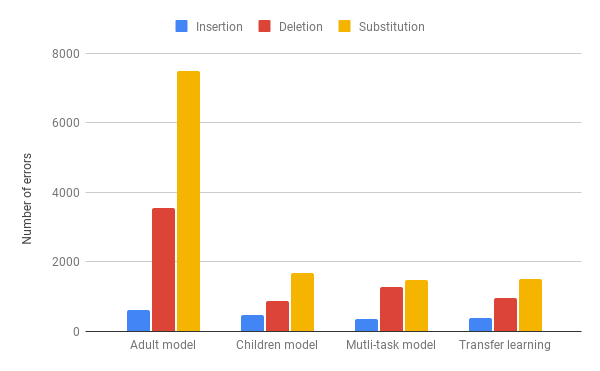
\includegraphics[scale=0.7]{imgs/IDS_HMM.png}
%        \caption{Type of error analysis depending on the model}
%        \label{fig:IDS_HMM}
%    \end{center}
%\end{figure}



\subsection{Summary and discussion}
% Conlusion
In this study, we conducted a knowledge transfer technique analysis to improve the results of ASR systems for children. We corroborate the acoustic mismatch between adult and child speech and the importance of the model encountering child data and its variability. Our investigations revealed that the transfer learning approach is a promising way to improve low-resource children's speech recognition scores. Furthermore, multi-task learning was found to be helpful in the setting of mixed adult-child ASR acoustic modelling.
% Open question for next section
However, in this study, we focus on the transfer from adults to children. It is not clear how such a system can work using only children's data.



\section{Combining multi-task and transfer learning using multilingual children data}
\subsection{Motivation}
% Explain motivation
In this section, we present our contribution, where we investigate the potential improvement in the performance of children's ASR for low-resourced languages by leveraging children's resources from various languages. Indeed, in many scenarios, both adults and children's speech data are limited or even unavailable. To overcome the challenges posed by substantial acoustic variability and data scarcity, we propose a novel approach that uses several small-sized corpora of children from diverse languages. Our study extends conventional multilingual training and transfer learning techniques for hybrid HMM-DNN ASR. We combine these techniques in a meaningful way to use knowledge from heterogeneous data sources. Initially, a multilingual model is trained using a multi-task learning objective, aiming to optimise network parameters for the distinct characteristics of children's speech across multiple languages simultaneously. Subsequently, this trained multilingual model is employed to enhance ASR performance for a target language. Note that the target language may be different from those included in the multilingual training stage. This is achieved through transfer learning, where the knowledge gained from the multilingual model is adapted to the specific characteristics of the target language. In our investigation, we aim to answer the following research question: \textit{Can these approaches be used to efficiently exploit low-resource children's speech data from multiple languages?} 

%In this section, we present our contribution where we study whether the performance of children's ASR for low-resourced languages may be improved by combining children's resources from different languages. In many scenario, there is limited or even no data for both adults and children. Therefore, we propose using several small-sized corpora of children from various languages to overcome the substantial acoustic variability and data scarcity issues. The current study extends standard multilingual training and transfer learning for hybrid HMM-DNN ASR by combining them in a meaningful way to use knowledge from heterogeneous data. First, a multilingual model trained with a multi-task learning objective tries to optimise network parameters to the specific characteristics of children's speech in multiple languages/tasks simultaneously. Subsequently, this multilingual model is used to improve ASR for a target language --potentially different from those used in the multilingual training stage-- by using transfer learning. We address the following research question: \textit{Can these approaches be used to efficiently exploit low-resource children's speech data from multiple languages?}

\subsection{The Multilingual-transfer learning approach}
\label{section:method}

We propose a new approach that combine transfer learning (TL) and multi-task learning (MTL) together for improved acoustic modelling of hybrid HMM-DNN ASR. The proposed approach consists of a two-stage procedure using both MTL and TL that extends the existing techniques since these are usually applied separately. First, a multilingual model trained with a multi-task learning objective attempts to optimise the network parameters to the particular characteristics of children's speech in multiple languages in parallel. In this work, the model is considered multilingual because all the tasks trained during multi-task learning are a corpus of children from  a different languages.
Secondly, we adapt this model for a specific children's corpus with TL. The motivation for using TL as a second stage is to take advantage of the robust pre-trained model trained during the MTL phase. Indeed, this pre-trained model has potentially learned cross-linguistic information about children's speech but has also seen more children's data than a model trained in a single language. 
For this purpose, the acoustic model is divided into two parts: the layers close to the input are shared across all languages and the top layers, close to the output, are language-specific. That is, there are as many output layers as there are languages, i.e. children corpora. Notice that one can incorporate a new language/task in this second stage by adding a new language-specific output,  even if this new language/task has not been seen during  MTL training (figure \ref{fig:MLTL1}).

Our hypothesis is that the more data from heterogeneous source seen by the acoustic model, the better the shared layers could capture the underlying characteristics of children's speech during the first stage of the procedure. These characteristics can be used effectively, later, by the language-specific layers and during the second step of the procedure (figure \ref{fig:MLTL1}). 

Although the approaches adopted in this work have been used previously in other studies, for instance \cite{TransferLF} and \cite{2019multi} where they successfully applied MTL using children speaking  Mandarin and English, obtaining a relative improvement of 16.96\% WER in the English children case, it is clear that successful performance of a methodological approach in the case of English cannot be expected to generalise to other contexts and languages.  
As we all know, English is a large-size, resource-rich pluricentric language which should be seen more as an exceptional case, rather than an average representative. Against this background, it is important to emphasise that there is a need for research that investigates whether methods that have already been tested for English also work in new contexts such as those of mid-sized languages with fewer resources than English, like Dutch, Portuguese, Swedish and German. 

\begin{figure}[t]
\begin{center}
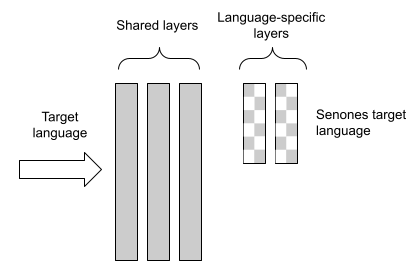
\includegraphics[scale=0.5]{imgs/Ours_final.png}
\caption{Multilingual transfer learning approach. Language-specific layers can be randomly initialised for a language not present during the MTL phase or use the corresponding pre-trained layers in case the target language was present during the MTL phase. Grey blocks are pre-trained during MTL phase.}
\label{fig:MLTL1}
\end{center}
\end{figure}


\subsection{Experimental Setup}
\label{section:corpus}
All experiments in this study were conducted using five children corpora, each representing a distinct language: PFSTAR\_SWE, ETLTDE, CMU, LETSREAD, and CHOREC. Detailed descriptions of these datasets are provided in Section \ref{section:children_corpora}. Table \ref{tab:statistics} offers statistics on the duration, number of utterances, and language of each corpus.

% Explain why not Myst 
It is important to note that, in this work, we deliberately focused on utilising small datasets to align with the typical size of available children's speech corpora. Consequently, the MyST children corpus, which is relatively large with over 100 hours of data, was not included in our experiments. More informations about this corpus can be found in section \ref{section:children_corpora}. Including MyST in this study would introduce bias toward American English in the multi-task setting, as it represents more than twice the cumulative duration of all our low-resource datasets. While there are ways to mitigate this bias, such as weighting the dataset contributions in the loss function, we chose not to explore this avenue in the scope of this thesis. Our emphasis on smaller datasets aims to better reflect the challenges associated with low-resource scenarios commonly encountered in children's speech research.


\begin{table}[ht]
\begin{center}
\begin{tabular}{llcc}
\hline
Corpus name & Language     & Train & Test  \\ \hline
\multicolumn{1}{l}{PFSTAR\_SWE} & Swedish             & 6030 utt  & 2879 utt  \\ 
\multicolumn{1}{l}{} &              & 04h00 & 01h48 \\\hline
\multicolumn{1}{l}{ETLTDE}      & L2 German   & 1445 utt &  339 utt \\ 
\multicolumn{1}{l}{}      &    &  04h41 & 01h06 \\ \hline
\multicolumn{1}{l}{CMU}         & English             & 3637 utt & 1543 utt \\ 
\multicolumn{1}{l}{}         &              & 06h26 & 02h45  \\ \hline
\multicolumn{1}{l}{LETSREAD}    & Portuguese & 3590 utt & 1039 utt \\ 
\multicolumn{1}{l}{}    &  & 12h00 & 02h30 \\  \hline
\multicolumn{1}{l}{CHOREC}      & Dutch               & 2490 utt & 575 utt  \\ 
\multicolumn{1}{l}{}      &                &  20h12 & 04h42 \\ \hline
\end{tabular}
\caption{Statistics on the different corpora of children's speech.}
\label{tab:statistics}
\end{center}
\end{table}


Our experimental design follows the same structure as the previous experiment, as outlined in Section \ref{section:exp_setup}. In this setup, the acoustic model is divided into two parts: the first part is shared across all languages, and the second part is language-specific. As each corpus represent a distinct language, we employ an independent language model and lexicon for each. Importantly, these language models and lexicons remain constant across all experiments to isolate the contribution of the acoustic model. Additionally, during the backpropagation process, all datasets are given equal weight contributions. 

\subsection{Multilingual-transfer learning experiment}

\begin{table*}[ht] 
\begin{center}
\begin{small}
\begin{tabular}{c|ccccc}

\hline
 & PFSTAR\_SWE & ETLTDE & CMU &  LETSREAD & CHOREC   \\  \hline
 \multicolumn{1}{c|}{Language} & \textit{Swedish} & \textit{German}  &  \textit{English}  & \textit{Portuguese} & \textit{Dutch}   \\ \hline
\multicolumn{1}{c|}{Single language} & 54.36\% & 44.69\%  &  21.26\%  & 26.88\% & 25.15\%    \\ \hline
\multicolumn{1}{c|}{MTL} & 54.95\% & 42.46\% & 23.01\% & 27.45\% & 25.10\%   \\ \hline
\multicolumn{1}{c|}{TL from PFSTAR\_SWE} & - & 42.23\% & 20.62\% & 26.47\% & 24.65\%   \\ 
\multicolumn{1}{c|}{TL from  ETLTDE}  & 53.60\% & -  &  20.90\% & 26.61\%  & 25.42\%        \\ 
\multicolumn{1}{c|}{TL from CMU}  & 52.83\%   & 41.54\%    & - & 26.49\% & 24.58\%   \\ 
\multicolumn{1}{c|}{TL from LETSREAD} & 52.50\% & 41.77\%  & 20.41\% & - & 24.60\%   \\ 
\multicolumn{1}{c|}{TL from CHOREC} & 52.20\% & 40.28\%    & 19.77\%    & 26.05\%   & -     \\ \hline
\multicolumn{1}{c|}{TL Average} & 52.78\% & 41.46\% & 20.43\% & 26.41\% & 24.81\%    \\ \hline
\multicolumn{1}{c|}{TL Best} & 52.20\% & 40.28\% & 19.77\% & 26.05\% & 24.58\%    \\ \hline \hline
\multicolumn{1}{c|}{MLTL} & \textbf{51.67\%} & \textbf{38.04\%} & \textbf{19.33\%} & \textbf{25.75\%} & \textbf{23.78\%}    \\ \hline \hline
\multicolumn{1}{c|}{MLTL-olo}  & \textbf{51.58\%} & 40.05\% & \textbf{19.67\%} & 26.20\% & \textbf{24.57\%} \\ \hline


\end{tabular}
\end{small}
\end{center}
\caption{WER results of multilingual-transfer learning and cross-lingual experiments. MTL: Multi-Task Learning, TL: Transfer Learning, MLTL: Multilingual Transfer Learning, MLTL-olo: Multilingual Transfer Learning one-language-out}
\label{tab:result-TL4epoch}
\end{table*}

Table \ref{tab:result-TL4epoch} presents the WER results of the multilingual transfer learning (MLTL) approach compared to three different methods: baseline, trained on each corpus individually for 4 epochs; Multi-task Training (MTL) alone, trained jointly using all corpora for 4 epochs; Transfer Learning (TL) alone, adapted for the target language using in turn one of the other 4 baseline models as a source, leading to 4 results per target language. In addition, for clarity, we summarise the transfer learning scores with the average of the 4 scores and the best of the 4 for each target.

Firstly, it is important to emphasise that the baseline scores correctly reflect the different tasks the children were asked to perform and the corresponding amount of data available for each corpus. The best WER score, 21.26\% for CMU, can be explained by the reading-aloud-sentences task nature of this corpus. Thus, the language model can more easily compensate for the acoustic model errors. In addition, Chorec and LetsRead, as the largest corpora in our experiment, also yield relatively good results for children's speech recognition. On the other hand, ETLTDE and PFSTAR\_SWE show the worse WER results with 44.69\%  and 54.36\% WER, respectively. This can be explained by the amount of data available and by the language model which does not compensate as much as the CMU model. Especially for ETLTDE, since it is the only corpus that does not contain scripted text, but spontaneous responses. In addition, the age range of PFSTAR\_SWE children also plays a critical role in performance, since younger children generally yield worse performance scores \cite{TFchildren}.

Turning to multi-task learning, among all the approaches presented, only MTL fails to improve the baseline performance for almost all languages, which is in contradiction with\cite{TransferLF}.  However, it can be explained by the differences in terms of the size of the child's speech corpora used. The smaller the size of the corpora used, the more difficult it is to model the acoustic variation in the children's speech.


Concerning TL, all performance scores outperform their corresponding baseline, confirming that TL is an adequate method for children's ASR since it allows the system to be confronted with more children, thus with more variation. Precisely, table \ref{tab:result-TL4epoch} shows that the best pre-trained model for knowledge transfer is Chorec.
This makes sense since Chorec is the largest corpus, representing about 40\% of the total data used in our experiments.


Finally, MLTL shows an average relative improvement in WER of 7.73\%  compared to the baseline, slightly higher than the average (TL Avg) and the best (TL Best) transfer learning performance, with an average relative improvement of 4.50\% and 2.66\%, respectively. 

The strength of MLTL is that it can benefit both from MTL and TL, minimizing some of their associated weaknesses.
Attending to our results, MTL does not improve single language training. We believe that the unbalanced amount of data, the significant differences among data sets and the use of segmental optimisation (lattice-free MMI) can partially explain these results. Nevertheless, we hypothesise that the multi-task objective leans the network towards 
better optimisation of the lower layers, rather than optimizing the upper language-specific layers, can still be beneficial for TL.
Regarding TL, one can observe considerable performance variations depending on the pre-trained model used as the source model, probably due to a poorer initialisation of lower layers that is less efficient for TL. The MLTL experiments show that we can overcome these drawbacks by combining both MTL and TL, thus, validating the effectiveness of this approach for robust speech recognition of children.



\subsection{Cross-lingual validation}
\label{section:olo}

In the previous section, we saw that the MLTL approach yields better results than separate multi-task and transfer-learning frameworks.

To further validate the hypothesis that the shared lower layers are able to learn meaningful information about children's speech characteristics, regardless of the language, we perform a cross-language experiment following a leave one-language-out cross-validation setting. In this experiment, we keep one language out of the multi-task training and use it only during the TL phase to adapt the acoustic model parameters. 

We repeated this procedure for each corpus in our experiment. As in the previous experiment, we used 4 epochs for each learning phase. The last row of Table \ref{tab:result-TL4epoch} presents the results of the cross-language experiment.

For all corpora, the MLTL one-language-out (MLTL-olo) approach outperforms the baseline WER score with an average relative improvement of 5.56\%. Improvements are more important for the small corpora ETLTDE and CMU, with a  relative improvement of 14.88\% and 9.07\%, respectively. PFSTAR\_SWE does not benefit as much, with only 5.05\% relative improvement. This is mainly due to the age differences with the children in the other corpora used in the MTL phase. Indeed, the children in PFSTAR\_SWE are much younger (see section  \ref{section:corpus} for more details). Therefore, we conclude that the shared layers have learned the underlying multilingual features of children.

It is also interesting to compare MLTL-olo with the results of transfer learning alone. In both cases, the pre-trained models used have never seen the target language data. We observe that the results between the MLTL-olo and TL Best are extremely close, with small improvement with the MLTL-olo, only the best transfer learning model on LetsRead is slightly better than MLTL. This means that during multilingual training the system learned, at least, the best representation of the available children's characteristics. This is consistent with our hypothesis of the important role of the multilingual training phase in our two-step procedure.

\section{Summary and discussion}
%\label{section:conclusions}
In this chapter, we have explored the current state of the art for Hybrid HMM-DNN speech recognition systems for children's speech. We aimed to address the following research questions: \textit{Which knowledge transfer approach is best for efficiently modelling and improving automatic recognition of children's speech? Can these approaches be used to efficiently exploit low-resource children's speech data from multiple languages?}.

Our results provide a positive response to these questions, first by demonstrating the effectiveness of knowledge transfer appraoch for children's ASR, particularly transfer learning. This efficacy arises from the ability of transfer learning to efficiently leverage knowledge encapsulated in a source pre-trained model trained on adult's speech. In addition, multi-task learning alone may not yield the most optimal results but we have demonstrated that the shared components of the model have the capacity to learn relevant information across multiple tasks jointly. Building on these insights, we propose a novel approach in this chapter—combining transfer learning and multi-task learning in our multilingual transfer learning system. We demonstrated that the challenges associated with both multi-task and transfer learning can be effectively overcome through our proposed approach. Indeed,this innovative system harnesses the strengths of the multi-task learning approach to learn pertinent information jointly, coupled with the efficiency of transfer learning in making effective use of pre-existing knowledge. Even in a low-resource scenario, this approach yielded promising results, resulting in an average relative improvement of 7.73\%. Additionally, the benefits of multilingual pre-training extended to transfer learning with an unseen language, showcasing an average relative improvement of 5.56\%. These findings underscore the suitability of multilingual transfer learning as a robust method for addressing children's speech recognition challenges, particularly in contexts with limited resources.

% Discussion
In the course of this chapter, our primary focus was directed towards the exploration of a multilingual system; however, it is crucial to emphasise the versatility of our approach. Indeed, our methodology could seamlessly be extended to various other tasks beyond multilingual scenarios. This extends to tasks involving age groups, accents, fluency levels, or varying degrees of intelligibility. It is worth noting that we did not extend our investigation to further scenarios within this thesis, primarily due to limitations in the available data corpora. Nonetheless, the extensibility of our approach holds promise for addressing a wide range of challenges across different linguistic and demographic dimensions in future research. In addition, as a future research direction , it would be interesting to investigate into the effects of incorporating a larger children's corpus, adult speech corpus or even non-European languages during the multilingual learning phase with specific weighting on the loss given previous studies' indication of performance improvements through the combination of large corpora from languages like Mandarin and English. Lastly, assessing the significance of the task's nature within both the multi-task learning and transfer learning phases offers a promising research direction. Understanding how different types of tasks or linguistic variations influence the model's adaptability.
%In future work, it would be interesting to investigate the effect of a larger children corpus or an adult speech corpus in the multilingual learning phase, as this would allow the model to be more acoustically robust. In addition, it would be interesting to explore the effect of non-European languages, as previous works has shown an improvement by combining Madarin and English. Furthermore, a more detailed comparison between age groups on the systems' performance would be an interesting next step. Finally, assessing the importance of the nature of the task within the multi-task phase and transfer learning phase would also be a possible avenue for future research.

% Transition to E2E
In the context of this thesis, we employed a TDNN-F based architecture within the different HMM-DNN systems developed in this chapter. This choice, acknowledged as the state-of-the-art for children's ASR in HMM-based systems, was motivated by previous research \cite{tdnnf-children}. However, in response to the emerging use of end-to-end ASR and the promising initial results observed for children's ASR, a strategic decision was made to transition towards the utilisation of end-to-end systems for the remainder of the thesis. This transition underscores an ongoing commitment to staying abreast of advancements in ASR methodologies and exploring innovative approaches that hold the potential to further enhance the recognition accuracy of children's speech.

